\documentclass[../main/journal_template.tex]{subfiles}
% This ties the document into the main file.  

% Don't put any packages here - if you want to include a package, put it in the main document header! 


% You can define local commands for this document: 
\newcommand{\fancyf}{\mathscr{F}}



\begin{document}
 
\section{Probability Theory}\label{sec:math_prob_thy}
% Note: You can label things locally and use \ref{}, \eqref{} etc, but referencing labels in *other* subfiles will only show up in the main document
\begin{itemize}
\item Citation: See Billingsley \cite{billingsley2008probability}
\item A fancy letter f: $\fancyf$
\item Local label reference: in this section (section \ref{sec:math_prob_thy}), we talk about probability theory. 
\item Global label reference: in another chapter, we talk about electrodynamics \ref{sec:physics_electrodyn}. Note that this label reference will only show up in the main document, not sub-files! 
\end{itemize} 

\section{Figures}
To include images, you can put them anywhere in the folder structure, but you have to give an absolute path relative to the base folder.  For instance, in the folder \verb|figures|, there is a picture called \verb|riemann.png|.  However, to include this image, I must use \verb|../math/figures/riemann.png| i.e. I have to go up to the main folder then back down.  This is so the main file will know where this image is.

\begin{figure}[ht]
\begin{center}
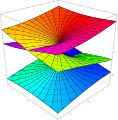
\includegraphics[scale=1]{../math/figures/riemann.png}
\end{center}
\caption{An illustration of a Riemann surface}
\label{somefig}
\end{figure}



% This is how to get bibliographies in both the sub-files and main document without double printing
\begin{comment}
\bibliographystyle{plain}
\bibliography{../main/journal_template_bib}
\end{comment}
\printbib{../main/journal_template_bib}
\end{document}